\section{Doc2Vec Modell}
\label{subsubsec:doc2vec}
In Anbetracht des unbefriedigenden Ergebnisses des DBScan-Algorithmus wird nun die Erprobung eines weiteren Modells in Betracht gezogen, um ähnliche Hotels zu identifizieren. Die nächste Alternative besteht in der Anwendung des Doc2Vec-Modells.
\newline
\newline
Doc2Vec ist ein maschinelles Lernverfahren, das dazu dient, Dokumente in einem kontinuierlichen Vektorraum abzubilden. Es wurde als Weiterentwicklung von Word2Vec konzipiert, einem etablierten Ansatz zur Repräsentation von Wörtern in einem semantischen Vektorraum. Das Hauptziel von Doc2Vec besteht darin, eine kontinuierliche Darstellung von Dokumenten zu generieren, um semantische Ähnlichkeiten zwischen diesen Dokumenten zu erfassen \cite{LeV.16.05.2014}.
\newline
\newline
Die grundlegende Idee besteht darin, jedes Hotel in einem textbasierten Dokument zu repräsentieren und dem Doc2Vec-Modell die Aufgabe zu übertragen, ähnliche Dokumente zu identifizieren. Dieser Ansatz zielt darauf ab, zu verhindern, dass Hotels ohne jegliche Zuordnung zu anderen Hotels vorliegen.
\newline
\newline
Ähnlich wie beim DBScan, wo der Vorteil darin bestand, keine Cluster angeben zu müssen, weist auch das Doc2Vec-Modell den Vorteil auf, dass keinerlei Cluster explizit angegeben werden müssen. Zudem eröffnet sich hier ein weiterer Vorteil, der beim DBScan-Algorithmus nicht gegeben war. Die beiden Informationen \emph{Art} und \emph{Region} sind beide durch Strings repräsentiert. Da Doc2Vec mit einer textbasierten Repräsentation arbeitet, bedarf es keiner Umwandlung dieser beiden Merkmale mittels \emph{One-Hot-Encoding}.

\subsection{Vorbereitung des Datensatzes} 
Auch in diesem Kontext erfordert der in Abbildung \ref{img:all_features_4} dargestellte Datensatz eine vorherige Verarbeitung, um mit dem Doc2Vec-Modell kompatibel zu sein. Die Vorbereitung besteht darin, dem Datensatz eine zusätzliche Spalte hinzuzufügen, die sämtliche Informationen des Hotels als textbasiertes Dokument repräsentiert. 
\newline
\newline
Im Folgenden wird eine Hilfsfunktion präsentiert, die dazu dient, die textbasierten Dokumente anhand der einzelnen Informationen zu erstellen.

\begin{lstlisting}[language=Python, label=lst:doc2vec_hilfs_func, caption=Hilfsfunktion zur Erzeugung von textbasierten Dokumenten]
# Copy the dataset to keep the original clean
doc2vec_df = df.copy()
    
# Get the columns of the dataset dynamic
column_names = doc2vec_df.columns
    
# Function to generate the document out of each columns
def concatenate_columns(row):
    result = "Hoteleigenschaften: "
    for column in column_names:
        result += column + "=" + str(row[column]) + " "
    return result
    
# Add the document in a new column "doc"
doc2vec_df['doc'] = doc2vec_df.apply(concatenate_columns, axis=1)
\end{lstlisting}

Durch die im Listing \ref{lst:doc2vec_hilfs_func} präsentierten Codezeilen, wurde dem Datensatz eine neue Spalte namens \emph{doc} hinzugefügt, die später als Eingabe für das Modell dienen soll. Zur Veranschaulichung dieser neu erstellten \emph{doc}-Spalte soll das erste Dokument als Beispiel dienen:

\begin{figure}[h]
    \centering
    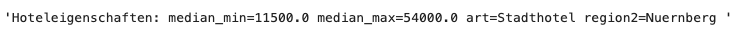
\includegraphics[width=1\textwidth, center]{ex_doc.png}
    \caption[Exemplarisches Dokument innerhalb des Datensatzes]{Exemplarisches Dokument innerhalb des Datensatzes}
    \label{img:ex_doc}
\end{figure}

Mithilfe dieser neuen Repräsentation kann nun im nächsten Schritt das Modell trainiert werden.

\subsection{Modellbildung}

Nach der erfolgten Datenvorbereitung und der Erstellung der textbasierten Dokumente für jedes Hotel kann das Modell nun trainiert werden. Hierzu werden die Hotel-IDs zunächst als Index festgelegt. Anschließend wird der Datensatz in sogenannte \emph{TaggedDocument} Objekte umgewandelt. Diese \emph{TaggedDocument} Objekte erfassen die einzelnen Wörter innerhalb eines Dokuments sowie ein sogenanntes \emph{Tag}, welches zur Identifikation des jeweiligen Dokuments dient. In diesem Kontext repräsentiert das \emph{Tag} die Hotel-ID. Der letzte Schritt besteht darin, die \emph{TaggedDocument} Objekte unter Verwendung einiger Hyperparameter dem Modell zuzuführen und das Training zu starten. Sobald das Modell trainiert ist, können ähnliche Dokumente zu einem ausgewählten Dokument, das durch die Hotel-ID identifiziert wird, gefunden werden.
\newline
\newline
Dieses Verhalten wird im nachfolgenden Listing dargestellt:
\begin{lstlisting}[language=Python, label=lst:doc2vec_exe, caption=Ausführung des Doc2Vec Modell]
# Generate the TaggetDocuments with Hotel-ID as Tag
documents = [TaggedDocument(words=doc.split(), tags=[str(i)]) for i, doc in doc2vec_df["doc"].iteritems()]
    
# Train the Model
model = Doc2Vec(documents, vector_size=10, window=3, min_count=1, workers=4, epochs=1000, alpha=0.01)
    
# Get similar documents als tupel (ID, Doc)
similar_documents = model.dv.most_similar(str(benchmark_hotel_id), topn=4)
    
pred_hotel_ids = [tupel[0] for tupel in similar_documents]
\end{lstlisting}

Nun stehen in der Variable \emph{pred\_hotel\_ids} die Hotel-IDs, die anhand von dem Doc2Vec Modell als am ähnlichsten empfunden wurden. Diese können wie auch schon beim DBScan Algorithmus anhand ihrer Merkmale betrachtet werden.

\begin{figure}[h]
    \centering
    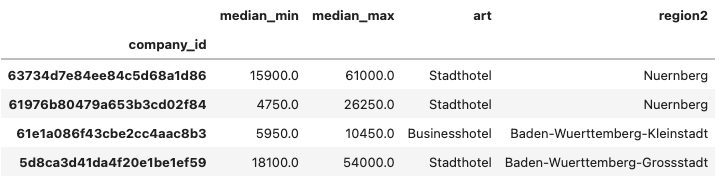
\includegraphics[width=1\textwidth, center]{doc2vec_hotels_1.png}
    \caption[Gefundene Hotels für das erste Benchmark-Hotel mit dem Doc2Vec Modell]{Gefundene Hotels für das erste Benchmark-Hotel mit dem Doc2Vec Modell}
    \label{img:doc2vec_hotels_1}
\end{figure}

Es zeigt sich, dass das Doc2Vec Modell ganz andere Hotels als ähnlich identifiziert hat. Im Gegensatz zum DBScan-Algorithmus scheinen die Merkmale der gefundenen Hotels lediglich Überlappungen aufzuweisen, anstatt sich zu teilen. Wie bereits in den vorhergehenden Abschnitten ersichtlich wurde, müssen sich die Merkmale nicht zwangsläufig überschneiden.

\subsection{Evaluation}
Ungeachtet der jeweiligen Merkmale der einzelnen Hotels besteht die Möglichkeit, dass diese dennoch Ähnlichkeiten in dem RevPAR-Verlauf aufweisen. Diese Annahme soll im Folgenden überprüft werden.

\begin{figure}[h]
    \centering
    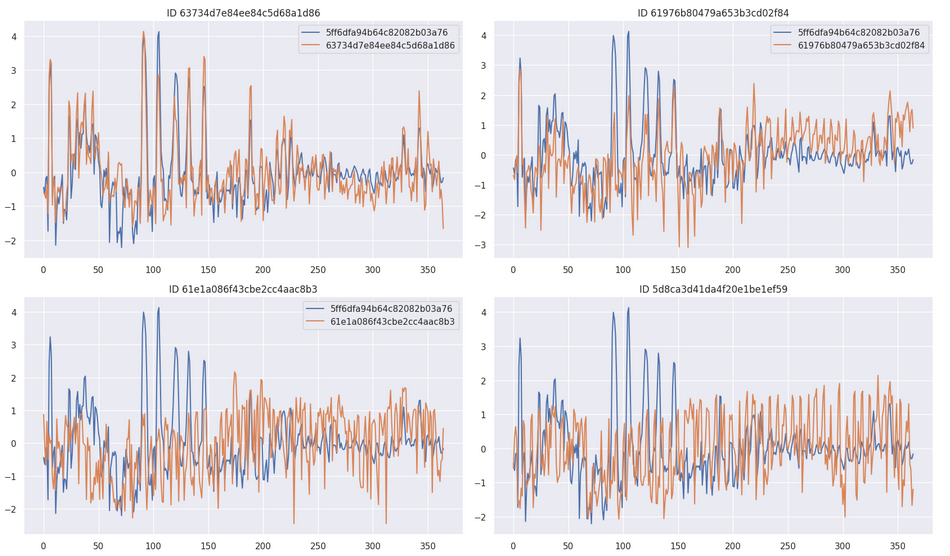
\includegraphics[width=1\textwidth, center]{doc2vec_results_1.png}
    \caption[Doc2Vec Ergebnisse der RevPAR-Verläufe für das erste Benchmark-Hotel]{Doc2Vec Ergebnisse der RevPAR-Verläufe für das erste Benchmark-Hotel}
    \label{img:doc2vec_results_1}
\end{figure}

\begin{figure}[h]
    \centering
    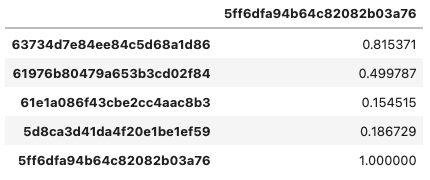
\includegraphics[width=0.5\textwidth, center]{doc2vec_results_1_1.png}
    \caption[Doc2Vec Ergebnisse der RevPAR-Korrelationen für das erste Benchmark-Hotel]{Doc2Vec Ergebnisse der RevPAR-Korrelationen für das erste Benchmark-Hotel}
    \label{img:doc2vec_results_1_1}
\end{figure}

Es offenbart sich, dass das Doc2Vec-Modell erheblich schlechter abschneidet als der DBScan-Algorithmus. Diese Feststellung wird bereits anhand des ersten Benchmark-Hotels ersichtlich, und es wird daher auf die detaillierte Evaluation dieses Benchmark-Hotels verzichtet.